	% !TeX encoding = UTF-8
% !TeX program = pdflatex
\documentclass[binding=0.6cm,LaM]{sapthesis}
\usepackage[utf8]{inputenx}
\usepackage{hyperref}
\hypersetup{pdftitle={Thesis},pdfauthor={Danilo Bernardini}}
\title{Design, development and evaluation of a framework for recording and synchronizing experiences in VR with physiological signals}
\author{Danilo Bernardini}
\IDnumber{1544247}
\course{Engineering in Computer Science}
\courseorganizer{Facoltà di Ingegneria dell'informazione, informatica e statistica}
\AcademicYear{2017/2018}
\copyyear{2018}
\advisor{Prof. Massimo Mecella}
%\coadvisor{Prof. Maurizio Caon}
\authoremail{danilo.bernardini93@gmail.com}
\begin{document}
\frontmatter
\maketitle
\tableofcontents
\mainmatter
\chapter{Introduction}

\chapter{Technologies}

This chapter introduces the involved technologies - virtual reality and physiological sensors -  and presents the current state of the art about them, including the available devices on the market and some application examples.

\section{Virtual Reality}
Virtual Reality (VR) is a technology that aims to allow a user to experience a computer-generated simulated environment. It commonly consists of a visual experience, but it can also include audio, haptic, touch and other feedback devices. 

Visual devices are usually VR headsets, head-mounted displays (HMD) with two screens - one per eye - that immerse the user in a virtual world simulating the real one. While wearing the headset, the user can look around rotating his head, move in the environment or interact with virtual objects using controllers, and perceive other senses through ad-hoc devices.

The above systems are usually computer-based, i.e. they are physically connected to the computer, so the applications run here and the visual output is transmitted to the headset display.
Another kind of solution is the one that uses the smartphone: in this case the headset is just a case that holds the device, the whole computation takes place in the smartphone and thus the applications are much simpler and less realistic compared to the computer-based ones (see \ref{sec:vrheadsets}).
	
\subsection{VR spread}
Virtual reality idea is not something new, there have been basic examples of it since the 1960s. The first head-mounted display system was the \textit{Sword of Damocles} \cite{sutherland1968head} created in 1968 by computer scientist Ivan Sutherland and his student Bob Sproull: the graphics were very primitive and consisted only of wireframe rooms, but the device was able to change the showed perspective according to the user head position. Its name comes from its appearance: the whole system was too heavy to be worn by a person so it was attached to the ceiling, suspended on the user's head.

In the next years different VR systems were developed, most of the times for the videogames industry. Examples can be found in some \textit{SEGA} and \textit{Nintendo} products. 

The main reason why VR is exploded in the last few years is that technology is now powerful enough to support advanced computation and to give users really immersive experiences. Until a few years ago VR solutions could not satisfy \textit{immersion} requirements (see section \ref{sec:measures}): graphics were not good enough and they had low refresh rates, causing the user some sickness (see section \ref{sec:measures}).

Conversely, in the present days we can rely on powerful machines and tools that allow us to create and experience good simulations of the world, most of the times without perceiving any issue.

VR spread is also encouraged by the release of not very expensive headsets (see section \ref{sec:vrheadsets}): a lot of people can now buy VR systems, either for development or entertainment, but also companies are starting to use them for business (see next section).

We can refer to \textit{Gartner Hype Cycle for Emerging Technologies} of 2017 \cite{hypecycle} to understand VR position in the market. Gartner is an American research and advisory company that provides IT-related insights and market analysis. The Hype Cycle is "a graphical depiction of a common pattern that arises with each new technology or other innovation" \cite{hypecycledef}, i.e. a chart that shows the maturity and social application of a technology. The plot is divided in five phases representing the stages of a technology life cycle: Innovation Trigger, Peak of Inflated Expectations, Trough of Disillusionment, Slope of Enlightenment, Plateau of Productivity. 
Gartner releases it every year and in 2017 they stated that transparently immersive experiences are one of the 3 most trending topics, together with AI everywhere and digital platforms, and that VR is currently in the fourth phase of the cycle. This means that VR applications are starting to be understood and adopted by companies, that methodologies and best practices are being developed and that the technology is beginning to spread to the potential audience.


\subsection{Applications}
Virtual Reality has many applications in different fields, from gaming and entertainment to education and healthcare. Here are some examples of industries that are using VR for improving and enhancing their work.

\begin{description}

\item[Business:] Companies can make clients experience virtual tours of business environments; they can test and show new products before releasing them or train their employees using VR.

\item[Culture and education:] VR can be used in museums and historical settings to recreate ancient sites, monuments, cities; it can be
very useful for teaching, since students can be immersed in what they are studying and better understand things (e.g. history, geography, astronomy).

\item[Games and entertainment:] Gaming and entertaining industry is probably the biggest adopter of VR, since this brings the player in a whole new level of immersion and realism; VR is also used in movies, sport and arts.

\item[Healthcare:] VR allows to simulate a human body, so that students and doctors can study and train on it; it can simulate a surgery or perform a robotic one, i.e. control a robotic arm remotely; it can be used to treat phobias and diseases.

\item[Military:] VR can be used to perform a combat simulation where soldiers can train and learn battlefield tactics; it can be also useful for flight simulation or medical training on the battlefield.  

\item[Science and engineering:] Virtual reality technology can help scientists to visualize and interact with complex structures, or it can be used by engineers to design, model and see something in 3D. 

\end{description}


\subsection{Measures}
\label{sec:measures}
The previous sections mentioned the words \textit{immersion}, \textit{realism}, \textit{sickness}, etc. These are concepts we can analyze and measure during VR experiences. 

\subsubsection{Immersion and presence}
There is a lot of confusion about the concepts of immersion and presence; some people think they are the same thing, some others mix them up. According to Mel Slater, immersion concerns \textit{what the technology delivers from an objective point of view. The more that a system delivers displays (in all sensory modalities) and tracking that preserves fidelity in relation to their equivalent real-world sensory modalities, the more that it is 'immersive'} \cite{slater2003note}. 
This means that immersion is something that can be determined and somehow measured in an objective way, depending entirely on the technology and not on the user. 
Presence, on the contrary, is a user-dependent concept, something that varies depending on the person, a human reaction to immersion: each person can perceive a different level of presence inside the same system and even a single user can perceive a different level of presence using the same system in different times, depending on the user's emotional state, past history, etc. \cite{bowman2007virtual}.
We can say that presence is both immersion and involvement: this regards the state of focus and attention of the user and depends on the interaction with the virtual world, the storyline, and other similar features of the experience.

\paragraph{Measuring immersion}
Since immersion is an objective concept depending only on technology, we can measure it evaluating how close the system video, audio and other features are to the real world \cite{bowman2007virtual}. For example if we consider visual source, we can identify some parameters that influence it: 
\begin{itemize}
\item field of view and field of regard, respectively the size of the visual field that can be viewed instantaneously and the total size of the visual field surrounding the user;
\item display size and resolution;
\item stereoscopy and head-based rendering, given by head tracking;
\item frame rate and refresh rate.
\end{itemize}

\paragraph{Measuring presence}
Presence is a subjective measure and is not easy to quantify. During the years some techniques have been developed and tested, the most used ones are the following \cite{sanchez2005presence}:

\begin{description}

\item [Questionnaires]
Users participate to the virtual experience and then answer a questionnaire about presence. The questions imply responses between two extremes (e.g. from "no presence" to "complete presence"). The problem with this approach is that asking questions about presence can affect the actual perception of the participant.

\item [Behavioral]
We can see evidence of presence if users in the virtual world behave as if they were in the real world. This can be triggered by events that cause a physical reaction on the participant, such as a movement reflex or a body rotation.

\item [Physiological signals]
This is a specialization of the previous approach: if we know how a person physiologically reacts to an event, and we can find the same reaction during a virtual event, then this is a sign of presence. This technique can only be used when we have well-known and easy to measure reactions, for example fear, so it is not ideal for calm and "boring" scenarios where nothing happens.

\item [Breaks in presence (BIP)]
A break in presence is an event that occurs when the user becomes aware he is in a virtual environment. This can happen if the visual stimuli starts to lag, if the graphics become low-quality, if the user touches a physical object from outside the VR experience, etc. This approach allows to know presence by analyzing the moments when BIP occur, and it is a good alternative to the physiological one because it can be used in every kind of environment (calm, stressfull,scary, and so on).

\end{description}

\subsubsection{Co-presence}
When more than one participant share the same virtual environment we can measure co-presence (also known as shared presence). It is the feeling that the other participants are really present and that the user is interacting with real people \cite{casanueva2001effects}. As well as presence, also co-presence is measured with questionnaires. It is not proven that co-presence is related to presence, because some studies \cite{tromp1998small, slater2000small} seem to find correlation between them and others \cite{casanueva2001effects} do not.

\subsubsection{VR sickness}
As anticipated, virtual reality can cause some sort of sickness to the user. The common symptoms are similar to motion sickness symptoms: general discomfort, nausea, sweating, headache, disorientation, fatigue \cite{cobb1999virtual}.
Sickness varies from person to person and it is usually caused by conflicts between perceived movement and actual movement: if the player walks in VR the eyes say he is walking while the ears do not detect any movement, creating confusion to the brain. Other aspects that can induce sickness are low refresh rate and poor animations: both these things have the same effect on brain, which processes frames at higher rates or expects better animations.

Since it is a subjective feeling, the most common way of measuring VR sickness is through questionnaires. The standard methodology for measuring sickness is the \textit{Simulator Sickness Questionnaire (SSQ)} by Kennedy, Lane, Berbaum and Lilienthal \cite{kennedy1993simulator}. 
An interesting alternative approach is to monitor the postural activity of the participant \cite{riccio1991ecological}: it seems that motion sickness is related to postural stability and that there are differences in postural activity between people who are experiencing sickness and people who are not.

\subsubsection{Situation awareness}
A general measure that applies also for VR is situation awareness. It consists in having the awareness of what is happening in the surrounding environment and what may happen in the future, being ready to handle the situation that will arise. A famous approach to measure it is the \textit{Situational Awareness Rating Technique (SART)} \cite{selcon1990evaluation} originally developed by Taylor and Selcon in 1990 for evaluating pilots. It is a post-trial questionnaire that asks the user to rate 10 dimensions with a number from 1 to 7.

\subsubsection{Workload}
Another measure that can be useful in VR is workload, meant as the effort needed to complete a task. The most used technique is the
\textit{NASA Task Load Index (NASA-TLX)} \cite{hart1988development}, a questionnaire divided in two parts: the first one consists of 6 rating subscales, the second one is a personal weighting of these subscales.


\subsection{VR headsets}
\label{sec:vrheadsets}	
This section presents the most important available VR devices, starting from the computer-connected (tethered) headsets and continuing with mobile ones. Finally, standalone VR devices are introduced. 

\subsubsection{Tethered VR headsets}
Computer-connected VR systems take advantage of the computing power of the machine they are connected to, so they can give the user complex environments and experiences. The headsets provide head tracking and motion tracking - generally through external base stations - so the user can move with 6 degrees of freedom (DOF) and can interact with the virtual world in a lot of possible ways. 

\begin{description}

\item[HTC Vive]
HTC Vive system consists of a headset, two controllers and two base stations to track body movements. The display has 90 Hz refresh rate and 110 degree field of view, with a resolution of 1080x1200 per eye. The base stations also track the controllers, allowing an advanced interaction with the virtual environment. Together with several sensors, the headset also includes a front-facing camera. In 2018 HTC launched the Pro version of the Vive, fitted with a higher-resolution display, attachable headphones and a second camera.

\item[Oculus Rift]
Oculus initiated a Kickstarter campaign in 2012 and in 2014 it was acquired by Facebook. The system includes two Touch controllers and the headset hardware is basically the same as the HTC Vive's one. Tracking is obtained with \textit{Constellation}, an optical-based tracking system that detects IR LED markers on the HMD and controllers.

\item[Sony PlayStation VR]
PlayStation VR is Sony's proprietary VR system only compatible with PlayStation 4. It supports only PS4 ad-hoc games but there is the possibility to play any other PS4 game like if it was on a very large screen. Headset display has a resolution of 960x1080 per eye, a 100 degrees field of view and a native refresh rate of 90 or 120 Hz. Regarding the controller input, the system supports both regular \textit{DualShock 4} or \textit{PlayStation Move} controllers. Players need a \textit{PlayStation Camera} to track the HMD and the Move controllers.

\end{description}

\subsubsection{Mobile VR headsets}

A mobile VR system consists of a case that holds the smartphone and two lens that separate the display in two parts, one per eye. Since the only available sensors are those included in the smartphone, these VR systems can not track body movements and therefore they can just count on 3 DOF (head rotation). Since they are generally simpler and less powerful than the tethered ones, mobile VR systems are usually quite cheaper.

\begin{description}

\item[Google Daydream View]
Daydream is the enhanced successor of the \textit{Google Cardboard}, a very basic cardboard-made headset with two lenses that turns the smartphone into a VR system. Daydream software is built into the Android operating system since the Nougat version. The package comes with a wireless touchpad controller that can be tracked with on-board sensors.

\item[Samsung Gear VR]
Gear VR is a system only compatible with some high-level Samsung devices, it contains a controller equipped with a touchpad and a motion sensor. The development was carried out by Samsung in collaboration with Oculus, which took care of the software distribution. 

\end{description}

\subsubsection{Standalone VR headsets}
Standalone headsets are a new type of VR systems that does not require a computer or a smartphone in order to work. Since they have almost the same technical specifications, these devices computing power can be compared to that of smartphones, even if they are optimized for VR applications.

\begin{description}

\item[Oculus Go]
This device was developed by Oculus in collaboration with Qualcomm and Xiaomi. The HMD has 3 degree of freedom and is equipped with a 5.5-inch display with a resolution of 1280x1440 per eye, a Snapdragon 821 processor and comes with a 32GB or 64GB storage. The system also includes a wireless controller. 

\item[Lenovo Mirage Solo]
Mirage Solo is a brand new device and it works with Google Daydream platform. Technically speaking, its display is similar to the Oculus Go's one but the device is powered by a Snapdragon 835 with a 4GB RAM and it has a better tracking system, that gives the headset 6 DOF (but only 3 for the controller).

\end{description}


\subsection{Tracking devices}	
Together with headsets, a lot of different sensors and devices can be used to enhance VR experience. The most significant improvement in interaction is probably tracking. Most HMDs have an integrated head tracking system that allows 6 DOF movement, and controllers are usually tracked making it possible to interact with the environment. However, there exist external systems that enable advanced tracking functionalities such as full body tracking, hand tracking or eye tracking.

\subsubsection{Body tracking}
Body tracking makes possible to follow movements of the whole body, included arms and legs. It is a technique often used in movies and videogames to animate digital characters in CGI (in this case it is known as \textit{motion capture}). There are several companies providing body tracking solutions, here follows a list of some of the most valuable products currently available.

\begin{description}

\item[HoloSuit]
It is a suit that allows full body motion tracking and capturing thanks to the many sensors it has embedded. It also provides haptic feedback and it is compatible with the most important operating systems and development environments (\textit{Unity}, \textit{Unreal Engine}).

\item[HTC Vive Trackers]
Trackers are small disc-shaped devices that work with HTC Vive and they can be attached to any real physical object in order to track its movements. They can be also connected to the user to obtain body tracking or to replace Vive controllers.

\item[Optitrack]
Optitrack is one of the largest motion capture companies in the world, providing powerful tools and devices able to track small markers from long distances.

\item[Perception Neurons]
This system is composed of small units called Neurons that are placed to the various parts of the body, for example to fully track a person 11 to 32 Neurons are required. It is compatible with most 3D modeling and animation programs.

\item[PrioVR]
PrioVR uses sensors attached to key points of the body to provide full tracking without the need of a camera. It comes with small controllers and it works with both Unity and Unreal Engine.

\item[Orbbec]
Orbbec produces long-rage depth cameras that can be used with the proprietary body tracking SDK to fully detect the human body. It works with Windows, Linux and Android.

\item[Senso Suit]
Senso Suit is a kit composed of 15 modules, each containing a sensor and a vibrating motor, that make it possible to achieve full body tracking.  SDK available for Unity, Unreal Engine, C++ and Android. 

\item[VicoVR]
VicoVR is a wireless device that provides full body tracking to mobile VR headsets without the need of body-attached sensors. The device look is similar to \textit{Microsoft Kinect} (discontinued) and is compatible with Android, iOS and the main mobile VR headsets.

\item[Xsens]
Another big name in tracking industry, Xsens provides a variety of solutions for full body tracking, including suits or strap-based sensors kits. It does not need a camera and works with almost every 3D animation program.

\end{description}

\subsubsection{Hand tracking}
Hand tracking is a complex aspect of artificial intelligence that allows to detect and track hand movements only with a camera, without the need of any controller or external device. Here are presented two devices and a software library capable of detecting hand movements.

\begin{description}

\item[LeapMotion]
LeapMotion tracking system is a camera that needs to be attached to a VR headset in order to track hands with a field of view of 135 degrees. It works with both HTC Vive and Oculus Rift.

\item[uSens Fingo]
Fingo consists of a camera similar to LeapMotion that works with both tethered and mobile VR headsets, but it is optimized for mobile. Currently it is only compatible with Unity.

\item[OpenCV]
OpenCV (Open source Computer Vision) is a software library that provides several computer vision features, including hand tracking. It is written in C++ but there exist wrappers for other programming languages.

\end{description}

\subsubsection{Eye tracking}
Eye tracking is the process of detecting eye position and gaze. It is usually implemented with lights and cameras that analyze eye movement and detect the direction of gaze. Eye tracking is used in a lot of different fields such as safety (for example in a car), advertising, marketing and psychology.

\begin{description}

\item[aGlass]
aGlass is an eye tracking module compatible with HTC Vive. It is composed of two lenses that are placed above the Vive lenses and provide low-latency eye tracking with a field of view of 110 degrees.

\item[Fove]
Fove is a VR headset with an incorporated eye tracking module. It is compatible with SteamVR and OSVR and supports both Unity and Unreal Engine.

\item[Pupil]
Pupil Labs produces binocular eye tracking add-ons for the leading VR headsets. It comes with open source software and it works with Unity. 

\item[Tobii]
Tobii proposes an hardware eye tracking development kit for HTC Vive or a retrofitted version of the Vive with an eye tracking integration. 

\end{description}

\section{Physiological signals}
Physiological parameters are vital signals that describe a person's functions and activities state. There exist many different physiological signals, measurable with a lot of different sensors and devices. This section presents a wide variety of physiological sensors, from cheap wearable devices to expensive professional kits.

\subsection{Wearable devices}

\begin{description}

\item[Empatica E4 Wristband]
Wearable band and app for visualization and analysis, it comes with mobile API and Android SDK. 

Sensors: photoplethysmogram (PPG), accelerometer, EDA, thermometer.

\item[EQ02 LifeMonitor]
Device that can be worn on the chest and that stores or transmits the data to a mobile phone or a computer.

Sensors: ECG, respiration, skin temperature, accelerometer.

\item[Helo LX]
Smartband and app, it is compatible with Windows, Android, iOS.

Sensors: heart rate, breath rate, blood pressure.

\item[Microsoft Band 2]
Smartband by Microsoft, it can also work with Cortana. The app is available for Android, iOS and Windows Phone.

Sensors: heart rate

\item[Polar H10]
Heart rate sensor to attach on the chest, it comes with an internal memory and it also works with third-party applications. 

Sensors: heart rate

\item[Xiaomi Mi Band 2]
Band mainly used to monitor fitness exercises and to track sleep activity. 

Sensors: accelerometer, heart rate

\end{description}

\subsection{Professional kits}

\begin{description}

\item[Biopack Systems]
Hardware and software platform that provides professional measurements and analysis for research and education. The main module can acquire up to 16 different channels but it has no internal memory and it needs an external power supply.

\item[BiosignalsPlux]
BiosignalsPlux makes research kits that include 4 or 8 sensors and a 4 or 8 channels wireless hub, which has internal memory and battery. It works with third parties applications and sensors and comes with  Android, C++, Python, Java and MATLAB APIs.

\item[Libelium MySignals]
Software (uses an includes box screen) or hardware (uses Arduino) versions, acquired data is sent to the cloud and can be visualized on the web or on the mobile app. Up to 18 different sensors can be connected to the system. Available SDK for the hardware version.

\item[MindMedia NeXus-10]
Wireless acquisition system that supports 8 different signals, it includes a software for visualization and synchronization, together with a SD card and a battery for ambulant recordings.

\item[Thought Technology Biofeedback System]
5 or 8 channels system, it comes with proprietary software for data visualization and includes a memory card for offline acquisitions.

\end{description}



%\section{Usability}



\chapter{Project concept}
This chapter introduces the project idea and the concepts behind it, starting from the use of VR combined with physiological signals and going towards use cases and project requirements.

\section{VR and physiological signals}
Virtual reality is a powerful tool not only for commercial use, but also for research. Since the beginning of its lifetime, in fact, people started to think that it could have been a good environment to test and study certain phenomenons, especially concerning human body and behavior. From the first VR basic prototypes to the advanced systems of these last years, researchers have conducted lost of experiments about people reactions and emotions with VR making use of physiological signals. The reason why virtual reality is so appropriate and useful for research is that it can simulate real situations, so it gives researchers countless opportunities: they can recreate real world environments, test new kinds of interaction, make people relive specific scenes, and so on. 

As mentioned above, for many years there have been many examples of studies about VR with the use of physiological signals. An early research paper dealing with this subject was the one about fear of flying written by Wiederhold and others and published in 1998 \cite{wiederhold1998fear}. The authors wanted to test if there are significant physiological differences between people who are afraid of flying and people who are not. In order to accomplish that, they studied the body responses of two groups of people, one suffering from a fear of flying and the other one not, while experiencing a virtual reality flight. They measured heart rate, peripheral skin temperature, respiration rate, sweat gland activity and brain wave activity. The results of the experiment were successful and they could conclude that there exist significant differences between these two groups of people. In addition, the authors also succeeded in reducing arousal of people with fear of flying making them experience the simulation for several times. 

The following year another research paper about VR and physiological signals was published by Cobb and others \cite{cobb1999virtual}. This was one of the first investigations about VR sickness (see \ref{sec:measures}): the authors examined effects and symptoms of virtual reality on people using several methodologies, including physiological parameters.

These examples are part of the several research studies conducted to analyze or treat specific phobias and diseases. More recent ones are, for example, those by Kuriakose and Lahiri \cite{kuriakose2015understanding} and by Seinfeld and others \cite{seinfeld2016influence}, published in 2015 and 2016, respectively. Both are about anxiety: the former aims at measuring anxiety level in adolescents with autism using physiological signals while being in VR, the latter examines the influence of music on anxiety induced by fear of heights in VR. 

Finally, we can include in this list a paper about the hand illusion in VR with temperature monitoring by Llobera and others \cite{llobera2013relationship} and one about reduction of pain and anxiety in dental procedures using VR distractions \cite{wiederhold2014clinical}.

\section{Idea and requirements}
There are many experiments and studies using virtual reality that also include physiological signals; the previous section presented some of them showing that VR applications are limitless and that using physiology with it can lead to important results.
There is a common aspect in all these kind of studies: if the researchers want to collect physiological data during a virtual reality experience, they need to set up everything. This means to find a way to follow the experiment, to see what the participant sees in VR, to store data and to be able to analyze it. All these things are possible only if the collected data - VR video, physiological signals and other available sources - are synchronized. This process implies a lot of effort from the researchers because they have to figure out how to design and realize it, wasting time they could invest in the actual research.

This leads to the basic motivation behind this thesis project: designing and implementing a framework for recording and synchronizing experiences in VR with physiological signals. The framework would be a useful tool for whoever wants to physiologically analyze a certain phenomenon in VR. Having a ready-to-use test environment would allow to save time and focus on the actual experiment, since the only required thing is to build the virtual scene and everything else is done by the framework.

\subsection{Use cases}
The project requirements come from use cases. We can imagine three cases that should cover the main phases of a research on the above topic. 

\begin{enumerate}

\item examiner wants to see in real-time what the participant sees;

\item examiner wants to record the experiment session;

\item examiner wants to replay the session.

\end{enumerate}

Let's analyze these points one by one in order to fully understand what the system should do.

\begin{enumerate}

\item Since the framework is designed for conducting VR researches with physiological signals, who conducts the experiment should be able to see what the participant sees in the virtual world in real-time and how the body reacts to the experience.

\item In addition to real-time monitoring, the examiner should be able to record the whole session including all the signals and streams he has. Once recorded, everything should be synchronized in order to be easily accessible and analyzable in the future.

\item The examiner should have the possibility to offline replay a previously recorded session, being able to see everything as it was during the real-time monitoring. In this replay mode there should be the possibility to find key moments in which some relevant event happened and to place a marker on it for a quick and easy analysis.

\end{enumerate}

The figure shows the UML Use Case Diagram representing what stated above. 

\begin{figure}[h]
\centering
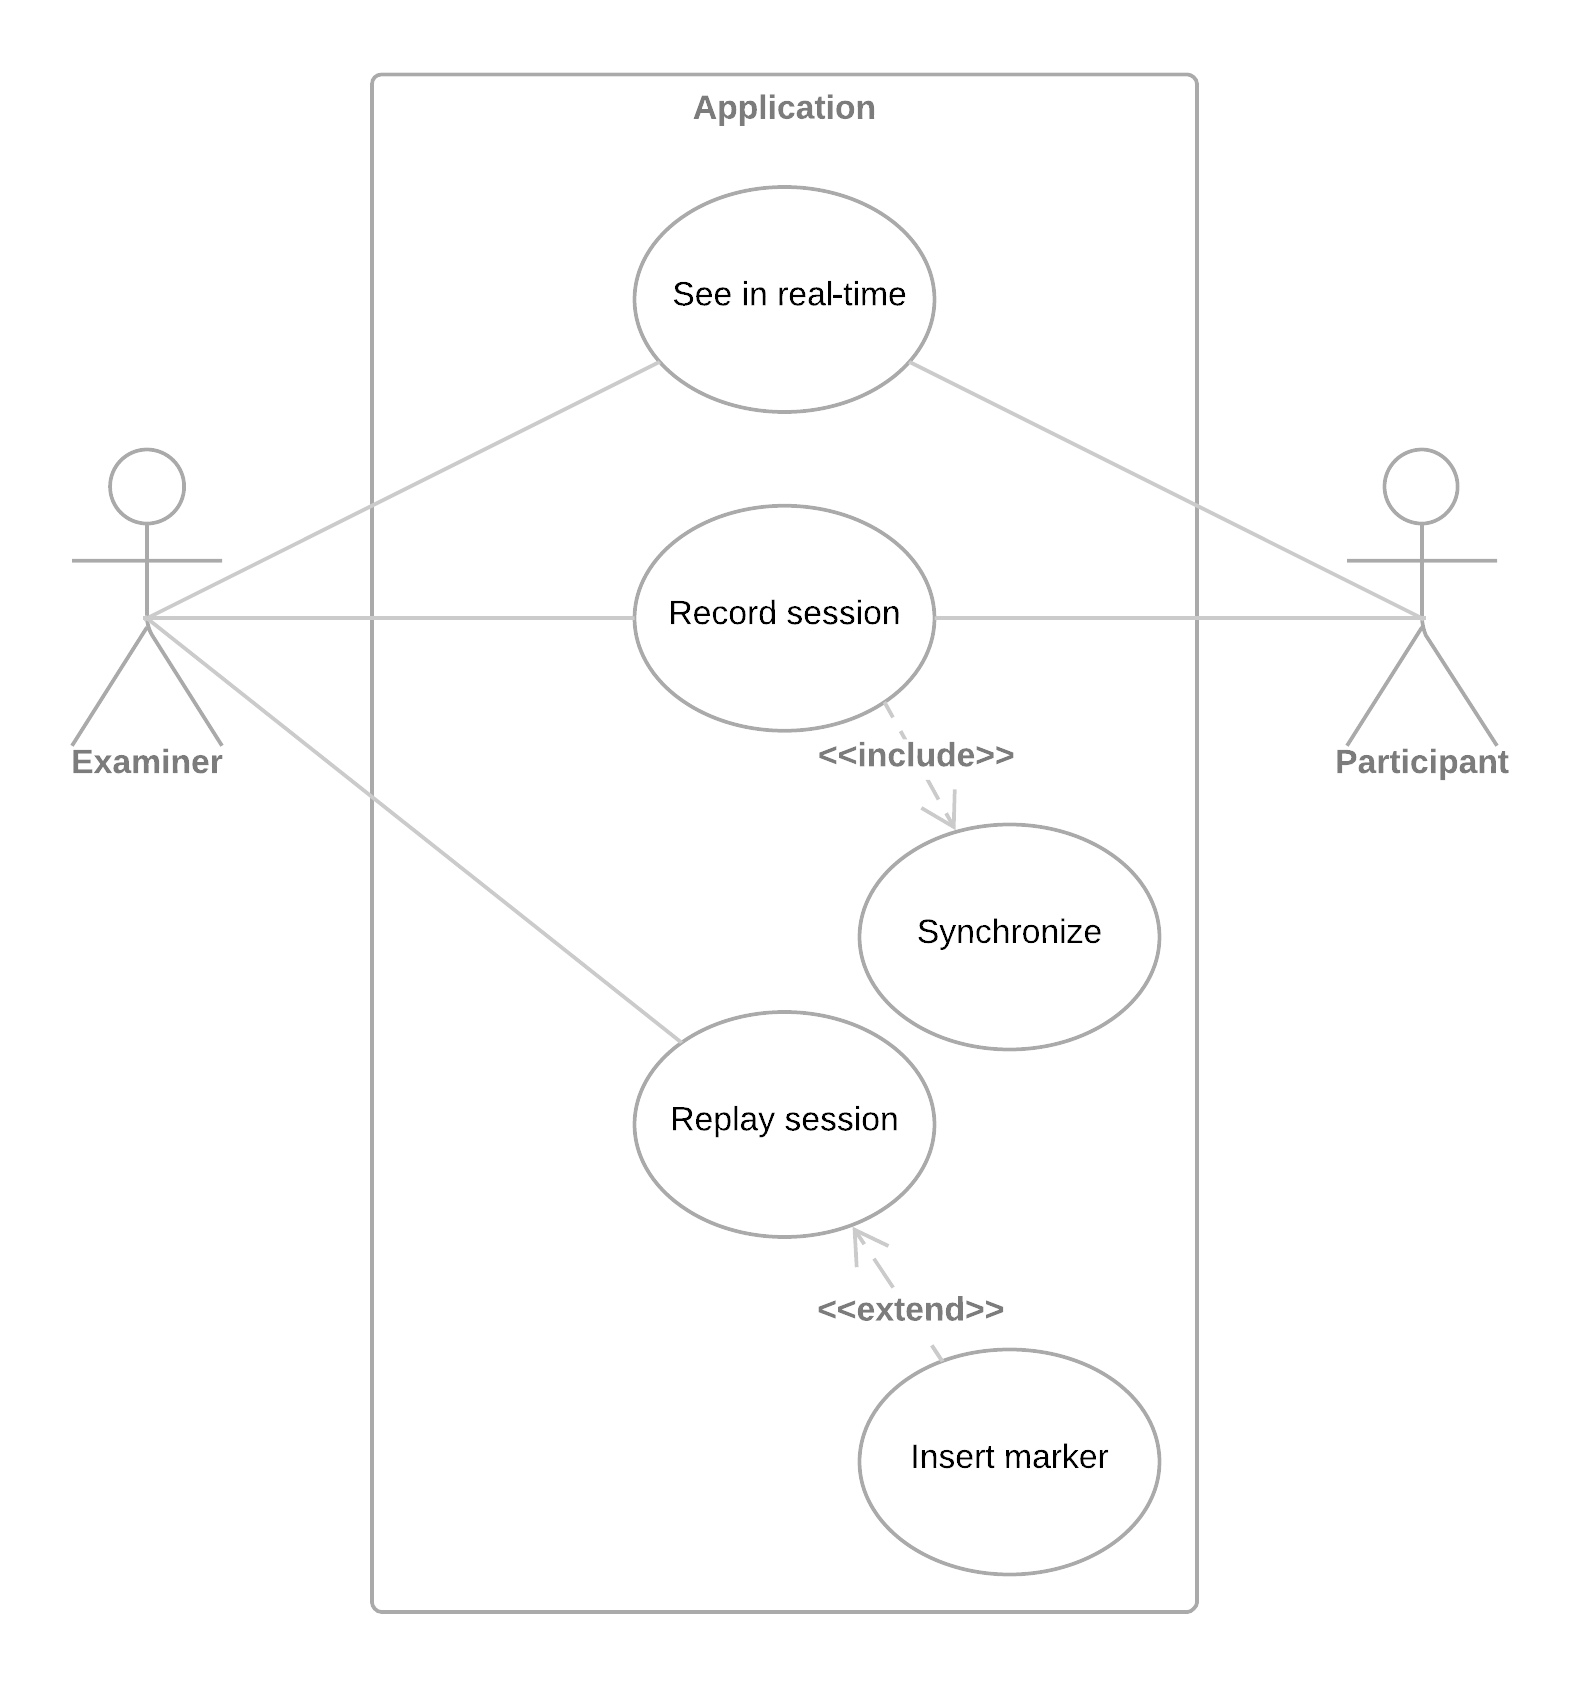
\includegraphics[scale=.257]{images/use_case_diagram_3}
\caption{Use Case Diagram}
\end{figure}

It is composed of two actors, the examiner and the participant, and three main use cases, reflecting the list above. The \textit{See in real-time} one is straightforward and is performed by both actors. The \textit{Record session} one is performed by both actors too, but it includes a sub-case: every time a session is recorded, it is also synchronized. \textit{Replay session} case instead is executed by the examiner alone at a later stage and it is extended by the \textit{Insert marker}, which is not mandatory.

\subsection{Requirements}
This section is about the requirements for the project, which result from the above use cases and from some other considerations. 

The system should allow to monitor a virtual reality experience while some sensors collect the participant's physiological signals. It would be reasonable to include in the system a camera that films the participant during the experience. This would make it possible to also have an external view on the user, being able to monitor his physical reactions to events. Examiners can see if the participant moves, rotates his body, is not stable, or has any other kind of reaction in response to a virtual stimulus.

Moreover, system structure and usability should not be hard, considering that the potential users will not be engineers or computer science experts. These people, in fact, will reasonably be scientist, doctors or researchers that need to test and analyze something in VR. 

The system should allow to to start a new real-time monitoring session which shows what the participant sees in VR, the camera source filming him and his physiological signals. During this "live" session, the examiner should be able to start a new recording: this will store the streams from VR, camera and sensors. At the end of the experiment the examiner should stop the recording and the various data need to be automatically synchronized. Alongside with the real-time mode, the system should have an "offline" part that allows to replay a previously recorded session. This mode should provide classical playback controls such as play, pause and stop, as well as timeline navigation to quickly skip to a specific frame. Since everything is already synchronized, in this modality the examiner can easily track every moment of the experiment; if there are relevant events it is worth to emphasize, the system should allow to place markers on them. 
Finally, the stored files (VR video, camera video and sensors data) should remain independent from each other, i.e. they should still be accessible from external programs after the synchronization and markers insertion.





\chapter{Design}

\section{Similar systems}

\subsection{Design}

\subsection{Physiological sensors}

\subsection{Connectivity and libraries}

\subsection{Events and triggers}

\subsection{Synchronization}

\subsection{Extensions}



\section{Design}


%\begin{figure}
%\centering
%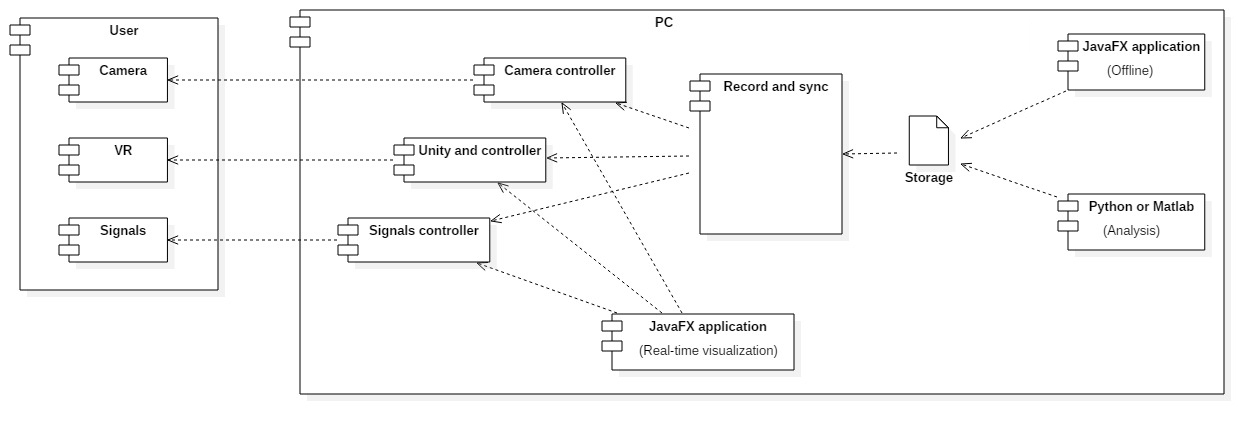
\includegraphics[scale=0.5,angle=90]{images/general_schema}
%\caption{General initial schema}
%\end{figure}

\chapter{Realization}
\section{Code snippets}

\section{Third parties software}



\chapter{Validation}
\section{Proof of concept test}

\subsection{Protocol}

\subsection{Results}

\section{Usability test}

\subsection{Protocol}

\subsection{Results}

\chapter{Conclusions}

\backmatter
\cleardoublepage
\phantomsection % Give this command only if hyperref is loaded
\addcontentsline{toc}{chapter}{\bibname}
\bibliographystyle{ieeetr}
\bibliography{bibliography}
\end{document}